\chapter{بخش ششم}
در این بخش به بررسی توانایی حذف اغتشاش 40 هرتز توسط برخی از کنترل‌کننده‌های منتخب از قسمت قبلی پرداخته می شود که بدین منظور نیز از نمودار bode تابع تبدیل مداربسته خروجی به ازای ورودی اغتشاش استفاده می شود که به صورت زیر می باشد:
$$
G_{d_i}^R = \dfrac{G}{1+K_{PIDF}G(1+K_{stabilizer})}
$$
عنوان نمونه نمودار bode تابع تبدیل معرفی شده در بالا به ازای کنترل‌کنندههای طراحی شده در فصل \ref{part_II} به صورت زیر می باشد: 
\begin{figure}[H]
	\centering
	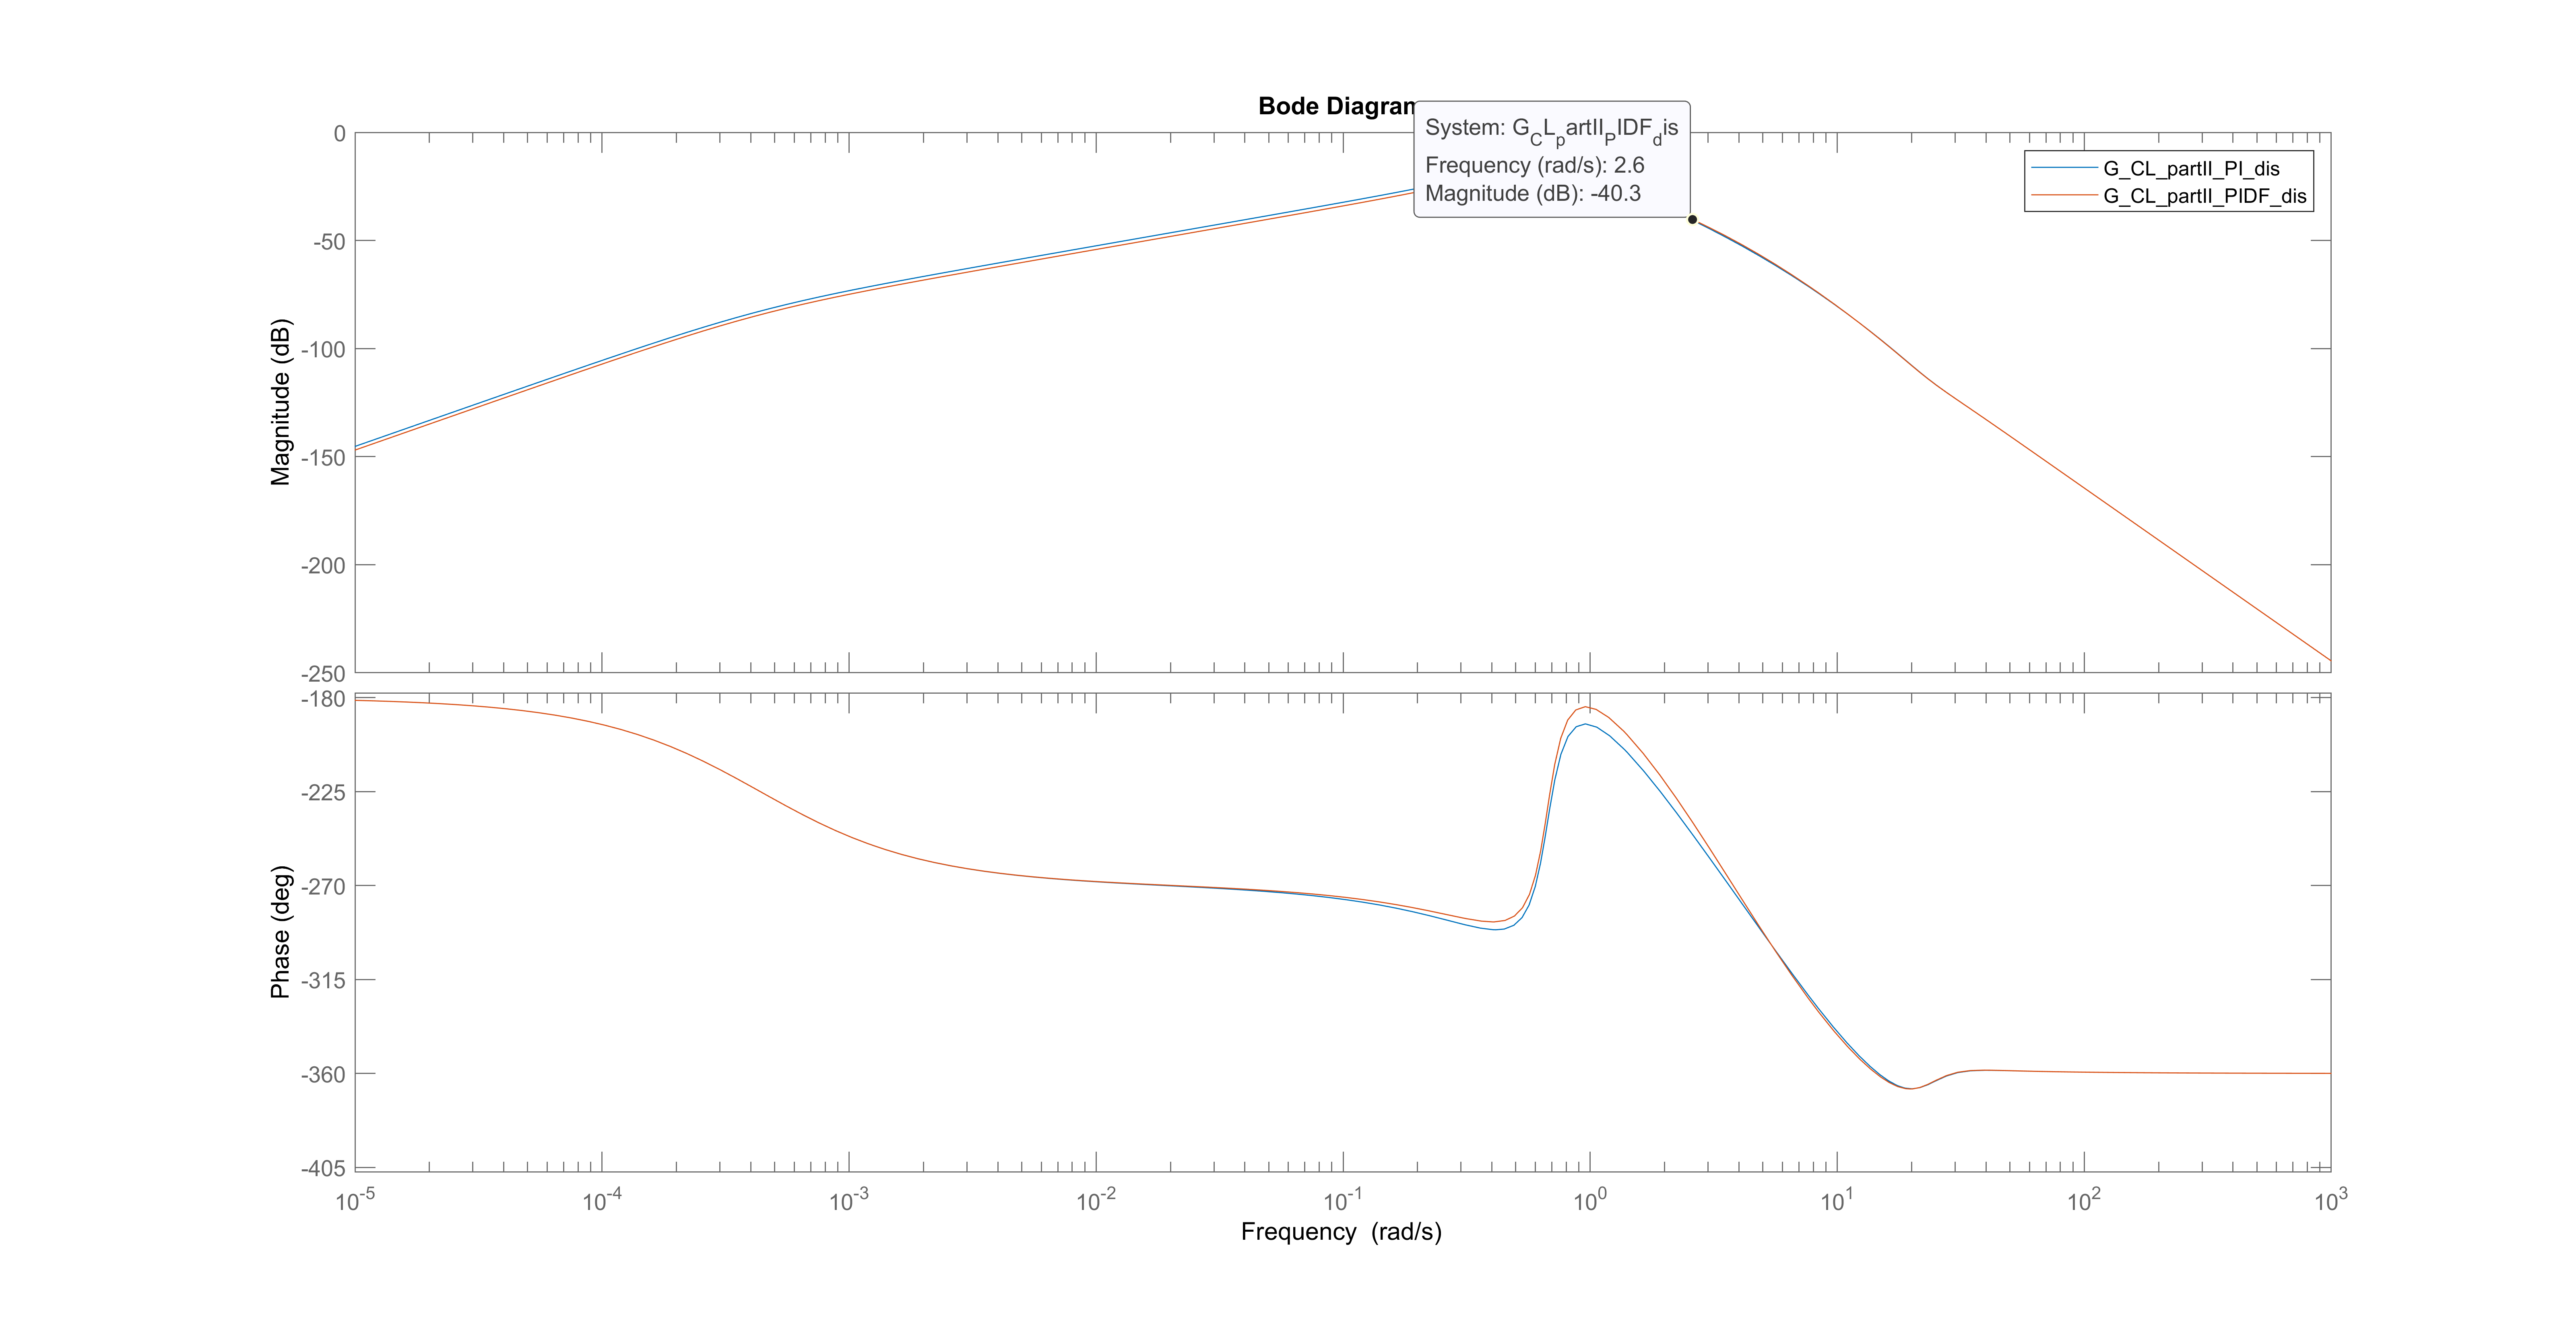
\includegraphics[width=12cm]{../Figure/P_VI/PID_tunner_dis_rej.png}
	\caption{‌دیاگرام bode تابع تبدیل خروجی به ورودی اغتشاش به ازای کنترل‌کنندههای طراحی شده به وسیله \lr{PID tunner}
	در بخش \ref{part_II}}
\end{figure}
همانطور که ملاحظه می شود دیاگرام بود در اغتشاش در این کنترل‌کننده ها در فرکانس 40 هرتز دارای اندازه -133  دسی بل می باشد که بیانگراین است که دامنه نواسانت در خروجی $2.2\times 10^{-7}$ برابر شده است که به معنی حذف کامل اغتشاش در فرکانس 40 هرتز می باشد.



برای کنترل‌کننده بخش
\ref{part_I}
نیز نمودار bode حلقه بسته کشیده شد که بر مانند کنترل‌کننده کاملا خواسته سوال را ارضا می‌کند.
\begin{figure}[H]
	\centering
	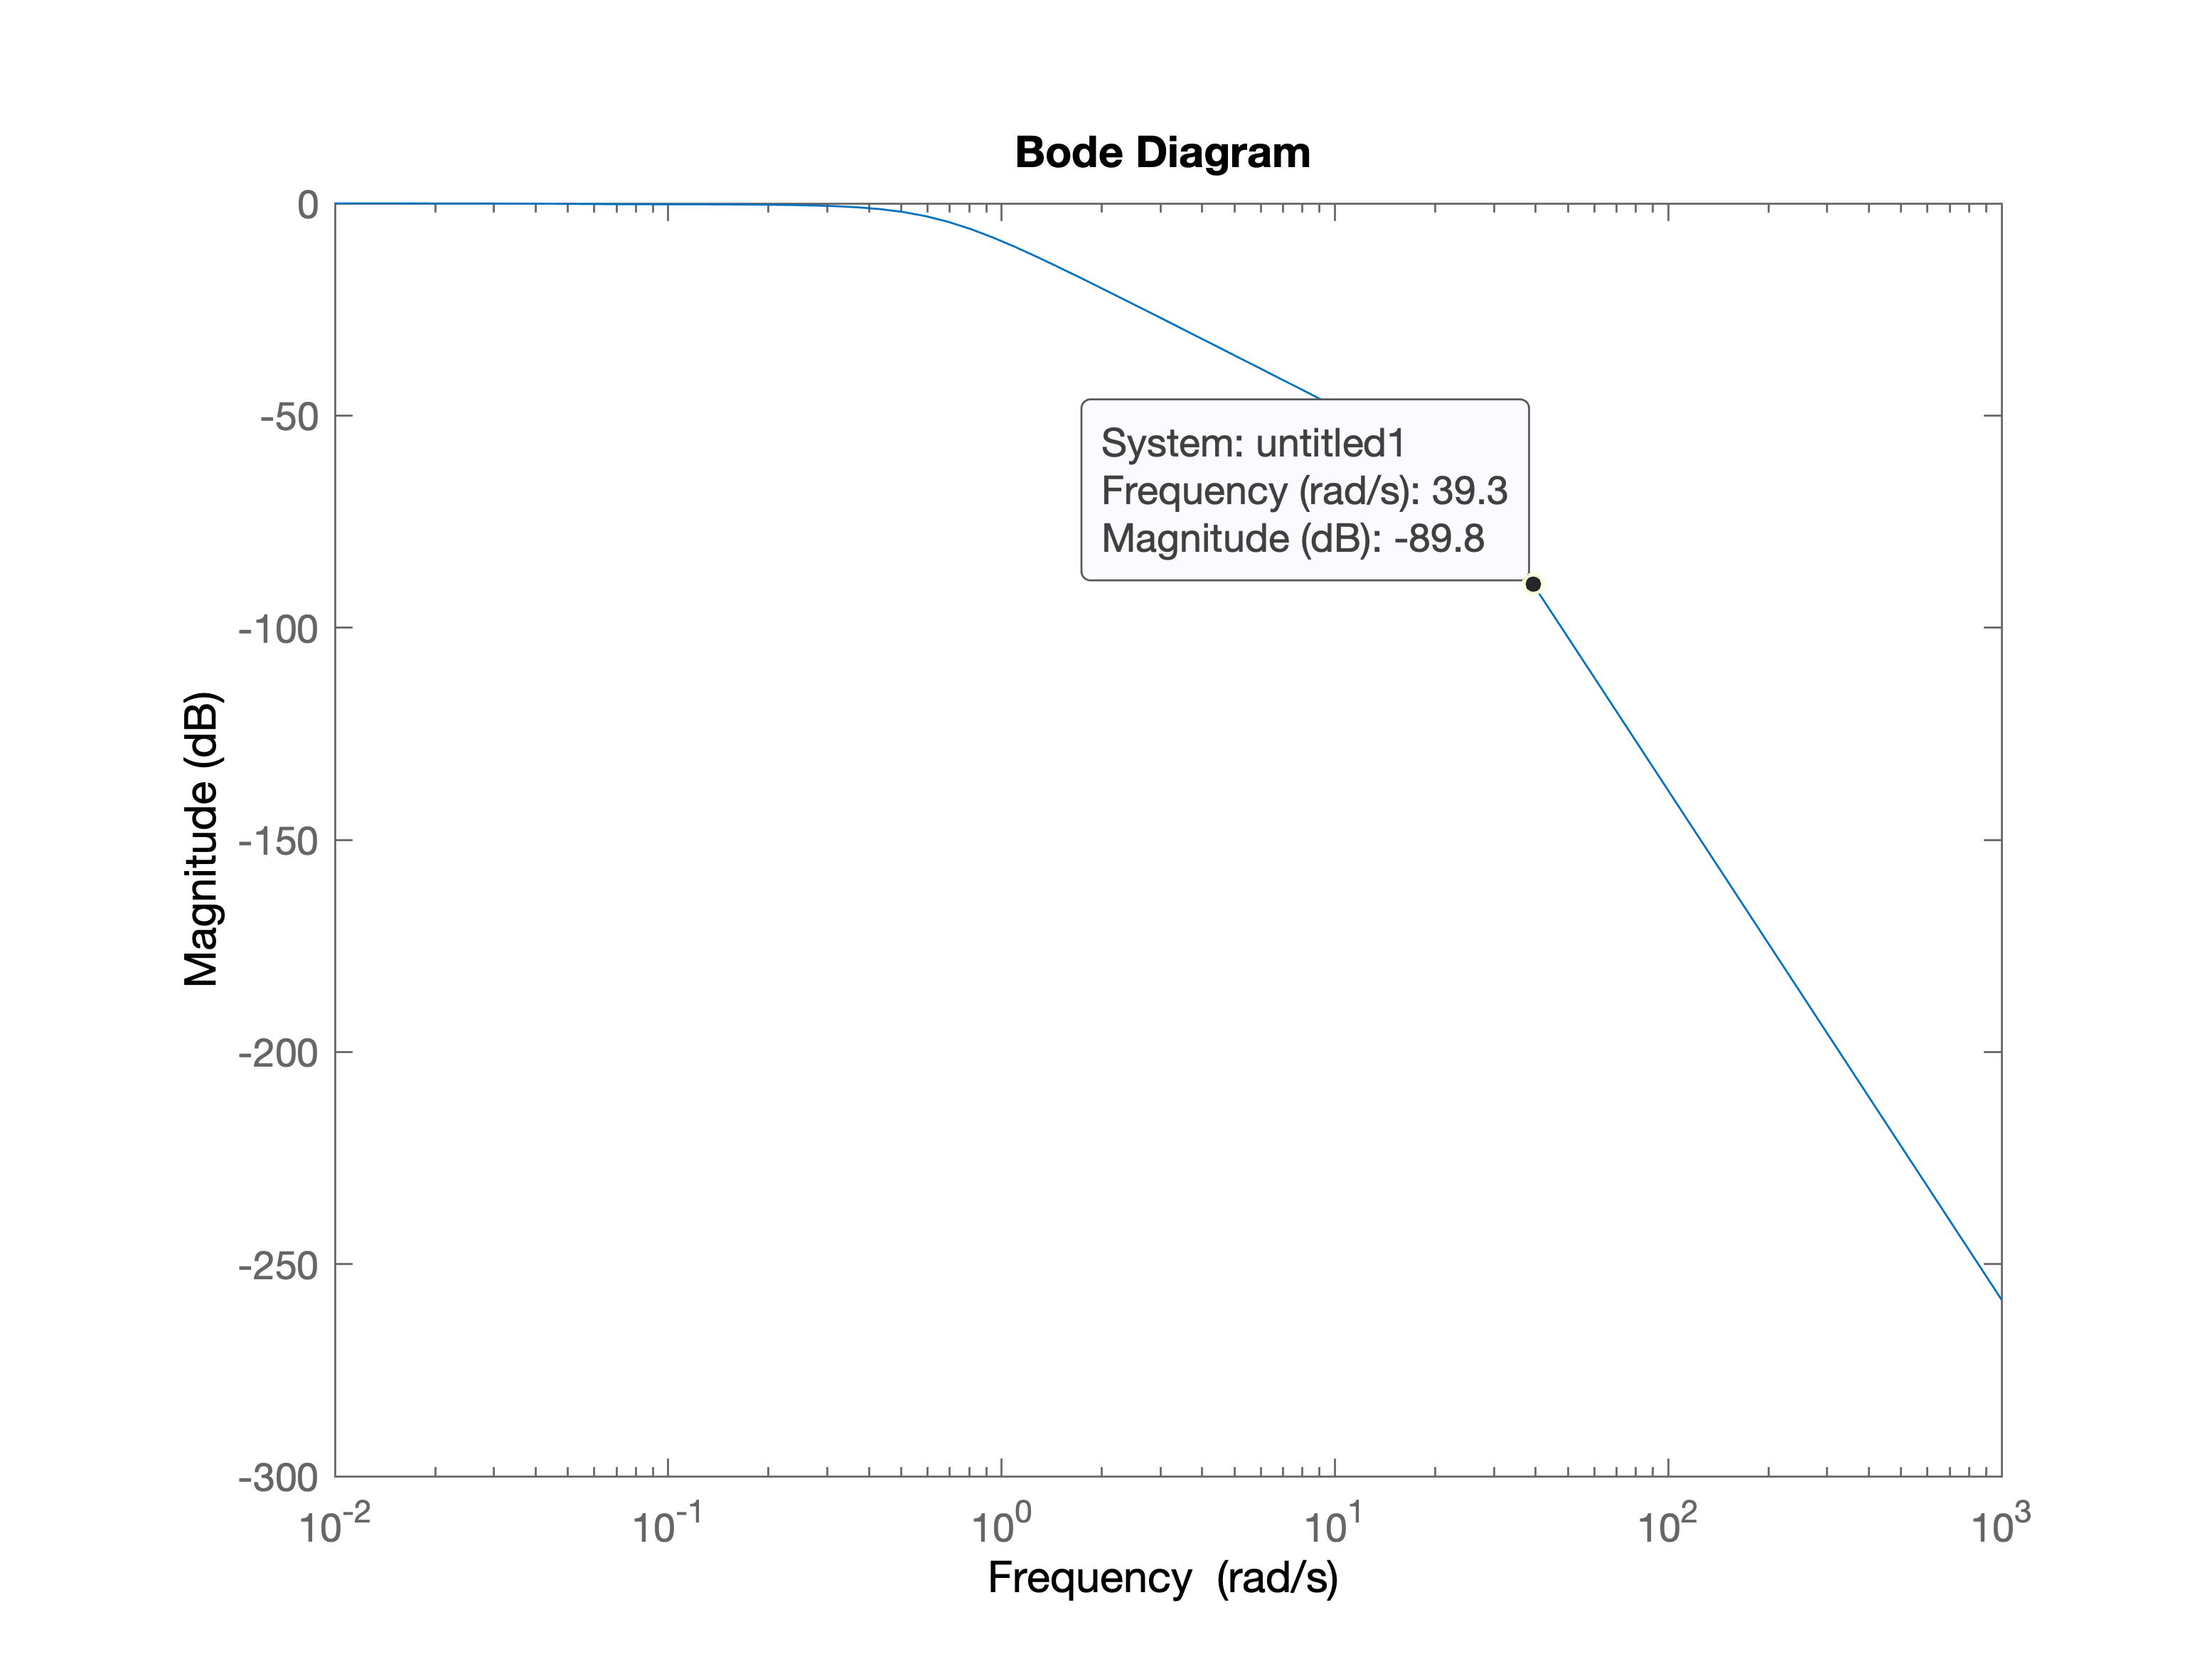
\includegraphics[width=12cm]{../Figure/P_I/PID_bode.png}
	\caption{‌دیاگرام bode تابع تبدیل خروجی به ورودی اغتشاش به ازای کنترل‌کنندههای طراحی شده به وسیله \lr{SISO tool PID}
		در بخش \ref{part_I}}
\end{figure}